% Created by tikzDevice version 0.12.3.1 on 2021-11-20 20:54:04
% !TEX encoding = UTF-8 Unicode
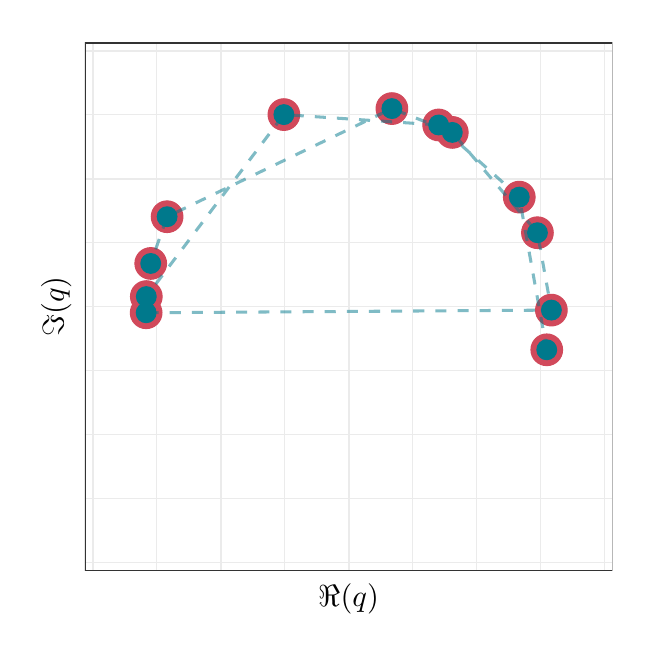
\begin{tikzpicture}[x=1pt,y=1pt]
\definecolor{fillColor}{RGB}{255,255,255}
\path[use as bounding box,fill=fillColor,fill opacity=0.00] (0,0) rectangle (216.81,216.81);
\begin{scope}
\path[clip] (  0.00,  0.00) rectangle (216.81,216.81);
\definecolor{drawColor}{RGB}{255,255,255}
\definecolor{fillColor}{RGB}{255,255,255}

\path[draw=drawColor,line width= 0.6pt,line join=round,line cap=round,fill=fillColor] (  0.00,  0.00) rectangle (216.81,216.81);
\end{scope}
\begin{scope}
\path[clip] ( 20.71, 20.71) rectangle (211.31,211.31);
\definecolor{fillColor}{RGB}{255,255,255}

\path[fill=fillColor] ( 20.71, 20.71) rectangle (211.31,211.31);
\definecolor{drawColor}{gray}{0.92}

\path[draw=drawColor,line width= 0.3pt,line join=round] ( 20.71, 46.70) --
	(211.31, 46.70);

\path[draw=drawColor,line width= 0.3pt,line join=round] ( 20.71, 92.91) --
	(211.31, 92.91);

\path[draw=drawColor,line width= 0.3pt,line join=round] ( 20.71,139.11) --
	(211.31,139.11);

\path[draw=drawColor,line width= 0.3pt,line join=round] ( 20.71,185.32) --
	(211.31,185.32);

\path[draw=drawColor,line width= 0.3pt,line join=round] ( 46.70, 20.71) --
	( 46.70,211.31);

\path[draw=drawColor,line width= 0.3pt,line join=round] ( 92.91, 20.71) --
	( 92.91,211.31);

\path[draw=drawColor,line width= 0.3pt,line join=round] (139.11, 20.71) --
	(139.11,211.31);

\path[draw=drawColor,line width= 0.3pt,line join=round] (185.32, 20.71) --
	(185.32,211.31);

\path[draw=drawColor,line width= 0.6pt,line join=round] ( 20.71, 23.60) --
	(211.31, 23.60);

\path[draw=drawColor,line width= 0.6pt,line join=round] ( 20.71, 69.81) --
	(211.31, 69.81);

\path[draw=drawColor,line width= 0.6pt,line join=round] ( 20.71,116.01) --
	(211.31,116.01);

\path[draw=drawColor,line width= 0.6pt,line join=round] ( 20.71,162.22) --
	(211.31,162.22);

\path[draw=drawColor,line width= 0.6pt,line join=round] ( 20.71,208.42) --
	(211.31,208.42);

\path[draw=drawColor,line width= 0.6pt,line join=round] ( 23.60, 20.71) --
	( 23.60,211.31);

\path[draw=drawColor,line width= 0.6pt,line join=round] ( 69.81, 20.71) --
	( 69.81,211.31);

\path[draw=drawColor,line width= 0.6pt,line join=round] (116.01, 20.71) --
	(116.01,211.31);

\path[draw=drawColor,line width= 0.6pt,line join=round] (162.22, 20.71) --
	(162.22,211.31);

\path[draw=drawColor,line width= 0.6pt,line join=round] (208.42, 20.71) --
	(208.42,211.31);
\definecolor{drawColor}{RGB}{209,73,91}
\definecolor{fillColor}{RGB}{209,73,91}

\path[draw=drawColor,line width= 0.4pt,line join=round,line cap=round,fill=fillColor] (187.57,100.41) circle (  5.71);

\path[draw=drawColor,line width= 0.4pt,line join=round,line cap=round,fill=fillColor] (177.64,155.58) circle (  5.71);

\path[draw=drawColor,line width= 0.4pt,line join=round,line cap=round,fill=fillColor] (148.50,181.65) circle (  5.71);

\path[draw=drawColor,line width= 0.4pt,line join=round,line cap=round,fill=fillColor] ( 92.58,185.40) circle (  5.71);

\path[draw=drawColor,line width= 0.4pt,line join=round,line cap=round,fill=fillColor] ( 42.87,119.64) circle (  5.71);

\path[draw=drawColor,line width= 0.4pt,line join=round,line cap=round,fill=fillColor] ( 42.81,113.79) circle (  5.71);

\path[draw=drawColor,line width= 0.4pt,line join=round,line cap=round,fill=fillColor] (189.24,114.75) circle (  5.71);

\path[draw=drawColor,line width= 0.4pt,line join=round,line cap=round,fill=fillColor] (184.20,142.72) circle (  5.71);

\path[draw=drawColor,line width= 0.4pt,line join=round,line cap=round,fill=fillColor] (153.44,178.96) circle (  5.71);

\path[draw=drawColor,line width= 0.4pt,line join=round,line cap=round,fill=fillColor] (131.61,187.57) circle (  5.71);

\path[draw=drawColor,line width= 0.4pt,line join=round,line cap=round,fill=fillColor] ( 50.38,148.50) circle (  5.71);

\path[draw=drawColor,line width= 0.4pt,line join=round,line cap=round,fill=fillColor] ( 44.46,131.61) circle (  5.71);
\definecolor{drawColor}{RGB}{0,121,140}

\path[draw=drawColor,draw opacity=0.50,line width= 1.1pt,dash pattern=on 4pt off 4pt ,line join=round] (187.57,100.41) --
	(177.64,155.58) --
	(148.50,181.65) --
	( 92.58,185.40) --
	( 42.87,119.64) --
	( 42.81,113.79) --
	(189.24,114.75) --
	(184.20,142.72) --
	(153.44,178.96) --
	(131.61,187.57) --
	( 50.38,148.50) --
	( 44.46,131.61);
\definecolor{drawColor}{RGB}{0,121,140}
\definecolor{fillColor}{RGB}{0,121,140}

\path[draw=drawColor,line width= 0.4pt,line join=round,line cap=round,fill=fillColor] (187.57,100.41) circle (  3.57);

\path[draw=drawColor,line width= 0.4pt,line join=round,line cap=round,fill=fillColor] (177.64,155.58) circle (  3.57);

\path[draw=drawColor,line width= 0.4pt,line join=round,line cap=round,fill=fillColor] (148.50,181.65) circle (  3.57);

\path[draw=drawColor,line width= 0.4pt,line join=round,line cap=round,fill=fillColor] ( 92.58,185.40) circle (  3.57);

\path[draw=drawColor,line width= 0.4pt,line join=round,line cap=round,fill=fillColor] ( 42.87,119.64) circle (  3.57);

\path[draw=drawColor,line width= 0.4pt,line join=round,line cap=round,fill=fillColor] ( 42.81,113.79) circle (  3.57);

\path[draw=drawColor,line width= 0.4pt,line join=round,line cap=round,fill=fillColor] (189.24,114.75) circle (  3.57);

\path[draw=drawColor,line width= 0.4pt,line join=round,line cap=round,fill=fillColor] (184.20,142.72) circle (  3.57);

\path[draw=drawColor,line width= 0.4pt,line join=round,line cap=round,fill=fillColor] (153.44,178.96) circle (  3.57);

\path[draw=drawColor,line width= 0.4pt,line join=round,line cap=round,fill=fillColor] (131.61,187.57) circle (  3.57);

\path[draw=drawColor,line width= 0.4pt,line join=round,line cap=round,fill=fillColor] ( 50.38,148.50) circle (  3.57);

\path[draw=drawColor,line width= 0.4pt,line join=round,line cap=round,fill=fillColor] ( 44.46,131.61) circle (  3.57);
\definecolor{drawColor}{gray}{0.20}

\path[draw=drawColor,line width= 0.6pt,line join=round,line cap=round] ( 20.71, 20.71) rectangle (211.31,211.31);
\end{scope}
\begin{scope}
\path[clip] (  0.00,  0.00) rectangle (216.81,216.81);
\definecolor{drawColor}{RGB}{0,0,0}

\node[text=drawColor,anchor=base,inner sep=0pt, outer sep=0pt, scale=  1.10] at (116.01,  7.64) {$\Re(q)$};
\end{scope}
\begin{scope}
\path[clip] (  0.00,  0.00) rectangle (216.81,216.81);
\definecolor{drawColor}{RGB}{0,0,0}

\node[text=drawColor,rotate= 90.00,anchor=base,inner sep=0pt, outer sep=0pt, scale=  1.10] at ( 13.08,116.01) {$\Im(q)$};
\end{scope}
\end{tikzpicture}
